% Gerado por gerar_dados_relatorio.js usando arrays_testados/resultados.csv.
% Não misturar com as medições diferentes do PDF usado como referência.
\section{Dados aleatórios}
\label{sec:aleatorio}
Apresentam-se as 9 dimensões registradas para dados aleatórios. R indica o recursivo, H o híbrido com pivô final e M3 o híbrido com mediana-de-três.
\begin{table}[htbp]
\centering\small
\caption{Tempo médio (ms) — dados aleatórios (R, H e M3)}
\label{tab:aleatorio:tempo}
\begin{tabular}{r r r r}
\hline
$n$ & R & H & M3 \\
\hline
100 & 0,14414 & 0,03118 & 0,07796 \\
500 & 0,11690 & 0,23998 & 0,12838 \\
1.000 & 0,27558 & 0,11922 & 0,21236 \\
2.000 & 0,16082 & 0,19418 & 0,46056 \\
5.000 & 0,52794 & 0,57604 & 0,99694 \\
10.000 & 1,14024 & 1,04510 & 1,10436 \\
20.000 & 2,42860 & 2,23888 & 2,17820 \\
50.000 & 6,16810 & 5,65368 & 5,96680 \\
100.000 & 14,45802 & 14,29448 & 11,11544 \\
\hline
\end{tabular}
\par\smallskip\footnotesize Fonte: arrays\_testados/resultados.csv; tempos convertidos de ns para ms. H e M3 usam $M=15$.
\end{table}
\begin{grafico}[H]
\centering
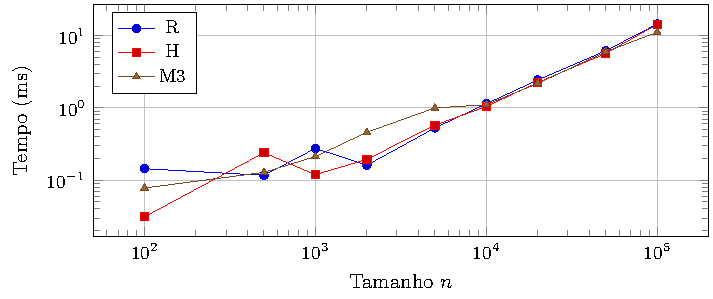
\includegraphics[width=.83\textwidth]{graficos/aleatorio_tempo.pdf}
\caption{Tempo médio por tamanho — dados aleatórios}
\label{graf:aleatorio:tempo}
\par\smallskip\footnotesize Fonte: arrays\_testados/resultados.csv. Eixos logarítmicos.
\end{grafico}
\begin{table}[htbp]
\centering\small
\caption{Comparações médias — dados aleatórios (R, H e M3)}
\label{tab:aleatorio:comparacoes}
\begin{tabular}{r r r r}
\hline
$n$ & R & H & M3 \\
\hline
100 & 595 & 636 & 640 \\
500 & 4.690 & 4.940 & 4.579 \\
1.000 & 10.481 & 10.972 & 10.373 \\
2.000 & 24.672 & 25.389 & 22.929 \\
5.000 & 70.861 & 73.162 & 65.611 \\
10.000 & 156.852 & 161.474 & 141.037 \\
20.000 & 338.200 & 347.730 & 303.752 \\
50.000 & 924.915 & 947.781 & 834.841 \\
100.000 & 1.943.232 & 1.988.771 & 1.799.683 \\
\hline
\end{tabular}
\par\smallskip\footnotesize Fonte: arrays\_testados/resultados.csv; contagens médias de operações. H e M3 usam $M=15$.
\end{table}
\begin{grafico}[H]
\centering
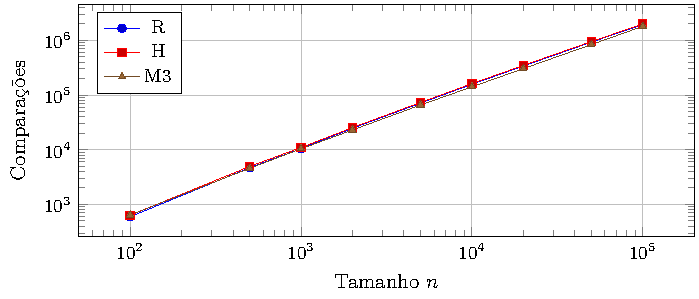
\includegraphics[width=.83\textwidth]{graficos/aleatorio_comparacoes.pdf}
\caption{Comparações médias por tamanho — dados aleatórios}
\label{graf:aleatorio:comparacoes}
\par\smallskip\footnotesize Fonte: arrays\_testados/resultados.csv. Eixos logarítmicos.
\end{grafico}
\begin{table}[htbp]
\centering\small
\caption{Trocas/movimentos médios — dados aleatórios (R, H e M3)}
\label{tab:aleatorio:movimentos}
\begin{tabular}{r r r r}
\hline
$n$ & R & H & M3 \\
\hline
100 & 244 & 416 & 414 \\
500 & 1.904 & 2.764 & 3.037 \\
1.000 & 5.473 & 7.091 & 6.913 \\
2.000 & 11.016 & 14.163 & 13.199 \\
5.000 & 32.696 & 41.103 & 36.987 \\
10.000 & 78.558 & 94.932 & 80.757 \\
20.000 & 152.928 & 186.977 & 175.539 \\
50.000 & 429.238 & 512.177 & 467.162 \\
100.000 & 883.375 & 1.049.788 & 1.003.896 \\
\hline
\end{tabular}
\par\smallskip\footnotesize Fonte: arrays\_testados/resultados.csv; contagens médias de operações. H e M3 usam $M=15$.
\end{table}
\begin{grafico}[H]
\centering
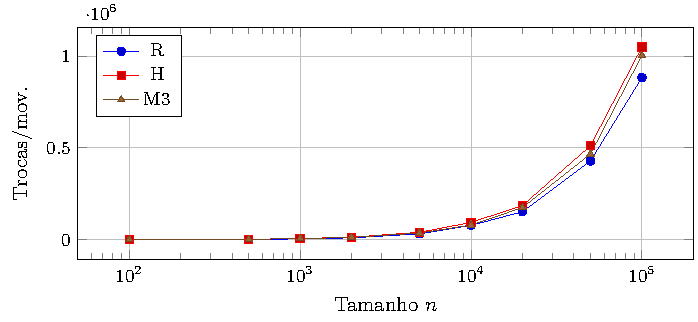
\includegraphics[width=.83\textwidth]{graficos/aleatorio_movimentos.pdf}
\caption{Trocas/movimentos médios por tamanho — dados aleatórios}
\label{graf:aleatorio:movimentos}
\par\smallskip\footnotesize Fonte: arrays\_testados/resultados.csv. Eixo horizontal logarítmico; zero preservado.
\end{grafico}
\subsection*{Interpretação: entrada aleatória}
As contagens crescem de milhares a milhões de comparações à medida que $n$ aumenta, sem a explosão quadrática determinística das entradas crescentes. Em $n=10.000$, R faz 156.852 comparações, H 161.474 e M3 141.037: a mediana reduz inspeções, mas H tem o menor tempo observado (1,04510 ms). Em $n=100.000$, M3 passa a ter menor tempo (11,11544 ms); H registra o maior número de trocas/movimentos (1.049.788 contra 883.375 de R). Isso é coerente com deslocamentos locais na inserção, não com trocas literais adicionais entre pares de posições. A não monotonicidade de tempos em alguns tamanhos (R passa de 0,27558 ms em 1.000 para 0,16082 ms em 2.000) recomenda não atribuir significado a diferenças pequenas sem dispersão e medições adicionais.

\section{Entrada crescente}
\label{sec:ordenado}
Apresentam-se as 6 dimensões registradas para dados crescentes. R indica o recursivo, H o híbrido com pivô final e M3 o híbrido com mediana-de-três.
\begin{table}[htbp]
\centering\small
\caption{Tempo médio (ms) — entrada crescente (R, H e M3)}
\label{tab:ordenado:tempo}
\begin{tabular}{r r r r}
\hline
$n$ & R & H & M3 \\
\hline
100 & 0,01412 & 0,01708 & 0,00196 \\
500 & 0,32652 & 0,36616 & 0,01086 \\
1.000 & 1,21644 & 1,21218 & 0,02226 \\
2.000 & 4,68986 & 5,43040 & 0,15874 \\
5.000 & 22,59508 & 23,17818 & 0,12780 \\
10.000 & 93,18666 & 83,49934 & 0,23122 \\
\hline
\end{tabular}
\par\smallskip\footnotesize Fonte: arrays\_testados/resultados.csv; tempos convertidos de ns para ms. H e M3 usam $M=15$.
\end{table}
\begin{grafico}[H]
\centering
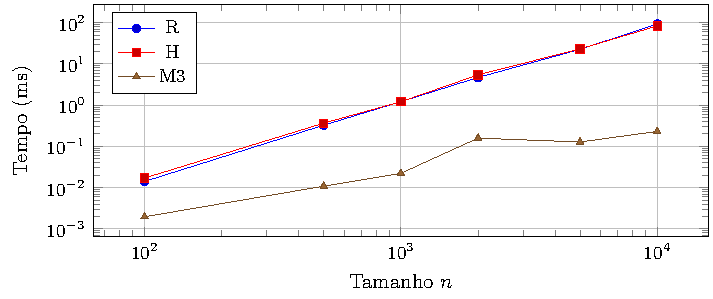
\includegraphics[width=.83\textwidth]{graficos/ordenado_tempo.pdf}
\caption{Tempo médio por tamanho — entrada crescente}
\label{graf:ordenado:tempo}
\par\smallskip\footnotesize Fonte: arrays\_testados/resultados.csv. Eixos logarítmicos.
\end{grafico}
\begin{table}[htbp]
\centering\small
\caption{Comparações médias — entrada crescente (R, H e M3)}
\label{tab:ordenado:comparacoes}
\begin{tabular}{r r r r}
\hline
$n$ & R & H & M3 \\
\hline
100 & 4.950 & 4.872 & 395 \\
500 & 124.750 & 124.672 & 3.288 \\
1.000 & 499.500 & 499.422 & 7.557 \\
2.000 & 1.999.000 & 1.998.922 & 17.094 \\
5.000 & 12.497.500 & 12.497.422 & 49.497 \\
10.000 & 49.995.000 & 49.994.922 & 108.986 \\
\hline
\end{tabular}
\par\smallskip\footnotesize Fonte: arrays\_testados/resultados.csv; contagens médias de operações. H e M3 usam $M=15$.
\end{table}
\begin{grafico}[H]
\centering
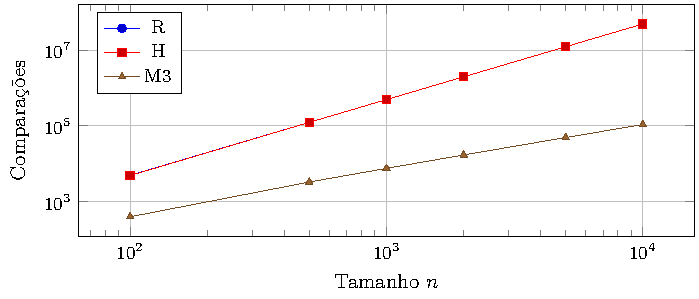
\includegraphics[width=.83\textwidth]{graficos/ordenado_comparacoes.pdf}
\caption{Comparações médias por tamanho — entrada crescente}
\label{graf:ordenado:comparacoes}
\par\smallskip\footnotesize Fonte: arrays\_testados/resultados.csv. Eixos logarítmicos.
\end{grafico}
\begin{table}[htbp]
\centering\small
\caption{Trocas/movimentos médios — entrada crescente (R, H e M3)}
\label{tab:ordenado:movimentos}
\begin{tabular}{r r r r}
\hline
$n$ & R & H & M3 \\
\hline
100 & 0 & 0 & 14 \\
500 & 0 & 0 & 104 \\
1.000 & 0 & 0 & 208 \\
2.000 & 0 & 0 & 416 \\
5.000 & 0 & 0 & 1.022 \\
10.000 & 0 & 0 & 2.046 \\
\hline
\end{tabular}
\par\smallskip\footnotesize Fonte: arrays\_testados/resultados.csv; contagens médias de operações. H e M3 usam $M=15$.
\end{table}
\begin{grafico}[H]
\centering
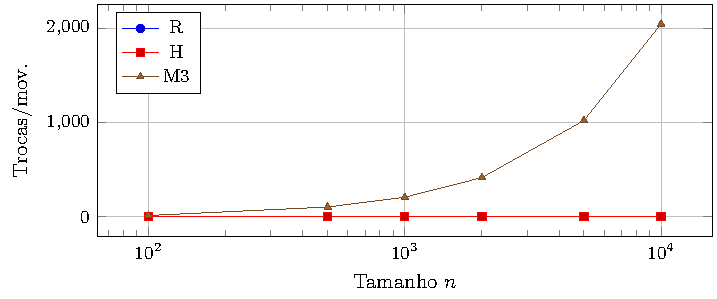
\includegraphics[width=.83\textwidth]{graficos/ordenado_movimentos.pdf}
\caption{Trocas/movimentos médios por tamanho — entrada crescente}
\label{graf:ordenado:movimentos}
\par\smallskip\footnotesize Fonte: arrays\_testados/resultados.csv. Eixo horizontal logarítmico; zero preservado.
\end{grafico}
\subsection*{Interpretação: entrada crescente}
No pivô final, cada varredura encontra o máximo da região; por isso R faz exatamente $n(n-1)/2$ comparações e nenhuma troca entre índices distintos. H elimina só 78 comparações em 10.000 valores, apesar do limiar de inserção, pois os subvetores grandes continuam degenerados. M3 escolhe inicialmente um valor central, reduzindo a profundidade efetiva nesta entrada; faz 108.986 comparações e 2.046 trocas/movimentos em 10.000 valores, contra 49.995.000 e zero de R. O resultado não significa que fazer mais trocas seja intrinsecamente melhor: o benefício decorre sobretudo de evitar milhões de inspeções nas partições desbalanceadas. A mediana não dá garantia de $O(n\log n)$ para entradas arbitrárias.

\section{Entrada decrescente}
\label{sec:inverso}
Apresentam-se as 6 dimensões registradas para dados decrescentes. R indica o recursivo, H o híbrido com pivô final e M3 o híbrido com mediana-de-três.
\begin{table}[htbp]
\centering\small
\caption{Tempo médio (ms) — entrada decrescente (R, H e M3)}
\label{tab:inverso:tempo}
\begin{tabular}{r r r r}
\hline
$n$ & R & H & M3 \\
\hline
100 & 0,00960 & 0,00758 & 0,00466 \\
500 & 0,12458 & 0,17294 & 0,01130 \\
1.000 & 0,52140 & 0,63826 & 0,02494 \\
2.000 & 2,03772 & 2,82486 & 0,06720 \\
5.000 & 14,27006 & 17,92168 & 0,15448 \\
10.000 & 60,29422 & 65,13762 & 0,61380 \\
\hline
\end{tabular}
\par\smallskip\footnotesize Fonte: arrays\_testados/resultados.csv; tempos convertidos de ns para ms. H e M3 usam $M=15$.
\end{table}
\begin{grafico}[H]
\centering
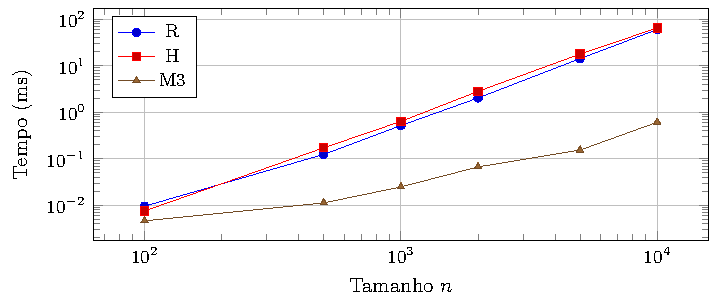
\includegraphics[width=.83\textwidth]{graficos/inverso_tempo.pdf}
\caption{Tempo médio por tamanho — entrada decrescente}
\label{graf:inverso:tempo}
\par\smallskip\footnotesize Fonte: arrays\_testados/resultados.csv. Eixos logarítmicos.
\end{grafico}
\begin{table}[htbp]
\centering\small
\caption{Comparações médias — entrada decrescente (R, H e M3)}
\label{tab:inverso:comparacoes}
\begin{tabular}{r r r r}
\hline
$n$ & R & H & M3 \\
\hline
100 & 4.950 & 4.950 & 878 \\
500 & 124.750 & 124.750 & 7.281 \\
1.000 & 499.500 & 499.500 & 16.783 \\
2.000 & 1.999.000 & 1.999.000 & 38.105 \\
5.000 & 12.497.500 & 12.497.500 & 109.138 \\
10.000 & 49.995.000 & 49.995.000 & 240.720 \\
\hline
\end{tabular}
\par\smallskip\footnotesize Fonte: arrays\_testados/resultados.csv; contagens médias de operações. H e M3 usam $M=15$.
\end{table}
\begin{grafico}[H]
\centering
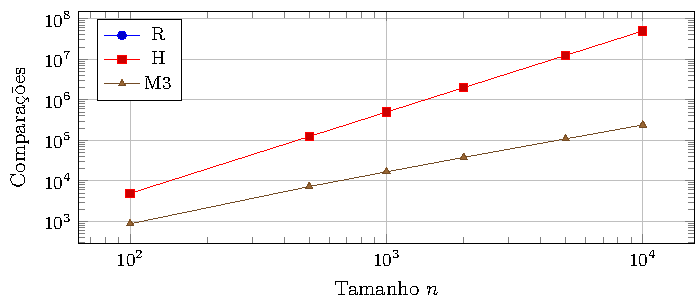
\includegraphics[width=.83\textwidth]{graficos/inverso_comparacoes.pdf}
\caption{Comparações médias por tamanho — entrada decrescente}
\label{graf:inverso:comparacoes}
\par\smallskip\footnotesize Fonte: arrays\_testados/resultados.csv. Eixos logarítmicos.
\end{grafico}
\begin{table}[htbp]
\centering\small
\caption{Trocas/movimentos médios — entrada decrescente (R, H e M3)}
\label{tab:inverso:movimentos}
\begin{tabular}{r r r r}
\hline
$n$ & R & H & M3 \\
\hline
100 & 50 & 147 & 567 \\
500 & 250 & 347 & 4.398 \\
1.000 & 500 & 597 & 9.622 \\
2.000 & 1.000 & 1.097 & 21.021 \\
5.000 & 2.500 & 2.597 & 55.627 \\
10.000 & 5.000 & 5.097 & 119.730 \\
\hline
\end{tabular}
\par\smallskip\footnotesize Fonte: arrays\_testados/resultados.csv; contagens médias de operações. H e M3 usam $M=15$.
\end{table}
\begin{grafico}[H]
\centering
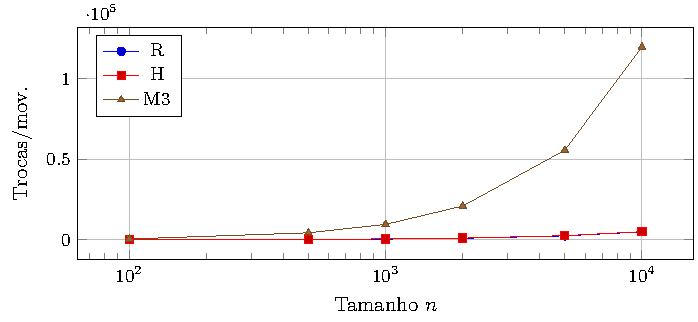
\includegraphics[width=.83\textwidth]{graficos/inverso_movimentos.pdf}
\caption{Trocas/movimentos médios por tamanho — entrada decrescente}
\label{graf:inverso:movimentos}
\par\smallskip\footnotesize Fonte: arrays\_testados/resultados.csv. Eixo horizontal logarítmico; zero preservado.
\end{grafico}
\subsection*{Interpretação: entrada decrescente}
O primeiro pivô final é mínimo, e os próximos pivôs permanecem extremos após as partições, levando novamente a $n(n-1)/2$ comparações em R. Diferentemente da entrada crescente, a posição final do pivô frequentemente difere de seu índice original: R registra 5.000 trocas em 10.000 valores; H registra 5.097 movimentos/trocas. M3 diminui as comparações para 240.720 e o tempo para 0,61380 ms, mas contabiliza 119.730 movimentações. A reorganização adicional é necessária para formar partições menos desiguais nesta implementação; tempo e número de movimentos não precisam variar na mesma proporção.

\section{Muitos valores repetidos}
\label{sec:duplicados}
Apresentam-se as 9 dimensões registradas para dados com duplicatas. R indica o recursivo, H o híbrido com pivô final e M3 o híbrido com mediana-de-três.
\begin{table}[htbp]
\centering\small
\caption{Tempo médio (ms) — muitos valores repetidos (R, H e M3)}
\label{tab:duplicados:tempo}
\begin{tabular}{r r r r}
\hline
$n$ & R & H & M3 \\
\hline
100 & 0,00206 & 0,00202 & 0,00228 \\
500 & 0,03054 & 0,00902 & 0,00784 \\
1.000 & 0,03646 & 0,03470 & 0,03760 \\
2.000 & 0,18880 & 0,07838 & 0,07304 \\
5.000 & 0,43580 & 0,25796 & 0,23756 \\
10.000 & 0,82768 & 0,71022 & 0,58158 \\
20.000 & 1,56256 & 1,36438 & 1,15740 \\
50.000 & 5,14288 & 4,38076 & 3,76142 \\
100.000 & 8,97956 & 8,04022 & 8,11022 \\
\hline
\end{tabular}
\par\smallskip\footnotesize Fonte: arrays\_testados/resultados.csv; tempos convertidos de ns para ms. H e M3 usam $M=15$.
\end{table}
\begin{grafico}[H]
\centering
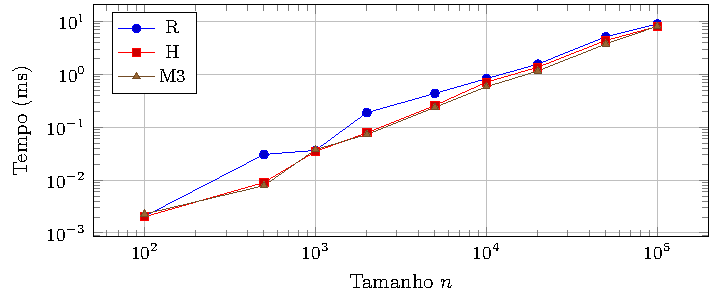
\includegraphics[width=.83\textwidth]{graficos/duplicados_tempo.pdf}
\caption{Tempo médio por tamanho — muitos valores repetidos}
\label{graf:duplicados:tempo}
\par\smallskip\footnotesize Fonte: arrays\_testados/resultados.csv. Eixos logarítmicos.
\end{grafico}
\begin{table}[htbp]
\centering\small
\caption{Comparações médias — muitos valores repetidos (R, H e M3)}
\label{tab:duplicados:comparacoes}
\begin{tabular}{r r r r}
\hline
$n$ & R & H & M3 \\
\hline
100 & 749 & 456 & 493 \\
500 & 5.768 & 4.372 & 3.883 \\
1.000 & 14.135 & 11.363 & 10.182 \\
2.000 & 30.732 & 25.016 & 21.355 \\
5.000 & 83.425 & 69.296 & 65.824 \\
10.000 & 167.611 & 139.666 & 144.327 \\
20.000 & 376.521 & 320.318 & 296.273 \\
50.000 & 1.008.325 & 867.115 & 776.512 \\
100.000 & 2.240.874 & 1.960.416 & 1.706.146 \\
\hline
\end{tabular}
\par\smallskip\footnotesize Fonte: arrays\_testados/resultados.csv; contagens médias de operações. H e M3 usam $M=15$.
\end{table}
\begin{grafico}[H]
\centering
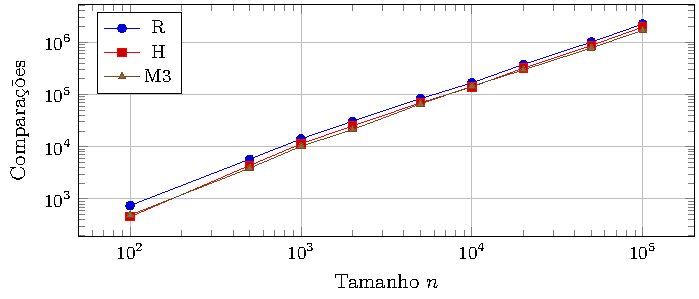
\includegraphics[width=.83\textwidth]{graficos/duplicados_comparacoes.pdf}
\caption{Comparações médias por tamanho — muitos valores repetidos}
\label{graf:duplicados:comparacoes}
\par\smallskip\footnotesize Fonte: arrays\_testados/resultados.csv. Eixos logarítmicos.
\end{grafico}
\begin{table}[htbp]
\centering\small
\caption{Trocas/movimentos médios — muitos valores repetidos (R, H e M3)}
\label{tab:duplicados:movimentos}
\begin{tabular}{r r r r}
\hline
$n$ & R & H & M3 \\
\hline
100 & 175 & 175 & 172 \\
500 & 1.835 & 1.961 & 2.092 \\
1.000 & 6.033 & 6.164 & 4.999 \\
2.000 & 8.928 & 9.131 & 8.893 \\
5.000 & 27.640 & 28.579 & 30.992 \\
10.000 & 60.102 & 62.072 & 61.848 \\
20.000 & 152.134 & 156.037 & 142.461 \\
50.000 & 367.209 & 375.556 & 340.456 \\
100.000 & 884.921 & 903.629 & 829.248 \\
\hline
\end{tabular}
\par\smallskip\footnotesize Fonte: arrays\_testados/resultados.csv; contagens médias de operações. H e M3 usam $M=15$.
\end{table}
\begin{grafico}[H]
\centering
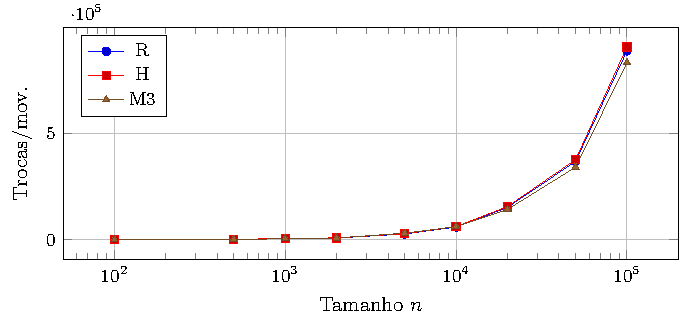
\includegraphics[width=.83\textwidth]{graficos/duplicados_movimentos.pdf}
\caption{Trocas/movimentos médios por tamanho — muitos valores repetidos}
\label{graf:duplicados:movimentos}
\par\smallskip\footnotesize Fonte: arrays\_testados/resultados.csv. Eixo horizontal logarítmico; zero preservado.
\end{grafico}
\subsection*{Interpretação: muitos valores repetidos}
Em 10.000 valores repetidos, M3 registra 0,58158 ms, abaixo de R (0,82768 ms) e H (0,71022 ms), embora H faça menos comparações que M3 (139.666 contra 144.327). Em 100.000, H supera M3 por apenas 0,07000 ms, sem que os dados disponíveis permitam declarar uma diferença confiável. O operador $\leq$ da partição coloca iguais à esquerda; a mediana entre três candidatos não separa uma região central de iguais. A quantidade de chaves possíveis cresce com $n$, portanto este ensaio não demonstra que todos os iguais seriam processados em $O(n\log n)$; uma partição em três vias seria uma extensão apropriada.

\section{Pior caso explícito}
\label{sec:pior}
Apresentam-se as 7 dimensões registradas para dados do pior caso explícito. R indica o recursivo, H o híbrido com pivô final e M3 o híbrido com mediana-de-três.
\begin{table}[htbp]
\centering\small
\caption{Tempo médio (ms) — pior caso explícito (R, H e M3)}
\label{tab:pior:tempo}
\begin{tabular}{r r r r}
\hline
$n$ & R & H & M3 \\
\hline
100 & 0,01050 & 0,00820 & 0,00128 \\
200 & 0,02352 & 0,03092 & 0,00240 \\
500 & 0,14554 & 0,28136 & 0,01004 \\
1.000 & 0,56778 & 0,77766 & 0,01532 \\
2.000 & 2,42954 & 3,53726 & 0,03578 \\
5.000 & 16,92574 & 25,46218 & 0,11224 \\
10.000 & 68,96428 & 82,97444 & 0,23330 \\
\hline
\end{tabular}
\par\smallskip\footnotesize Fonte: arrays\_testados/resultados.csv; tempos convertidos de ns para ms. H e M3 usam $M=15$.
\end{table}
\begin{grafico}[H]
\centering
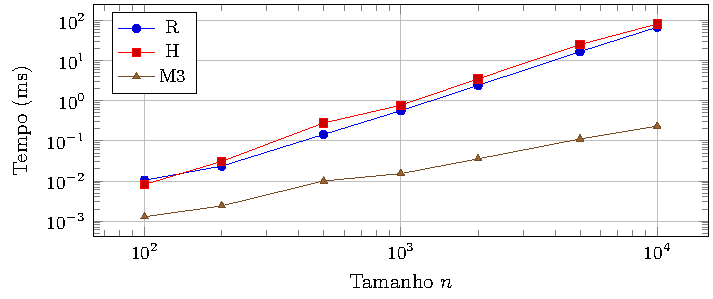
\includegraphics[width=.83\textwidth]{graficos/pior_tempo.pdf}
\caption{Tempo médio por tamanho — pior caso explícito}
\label{graf:pior:tempo}
\par\smallskip\footnotesize Fonte: arrays\_testados/resultados.csv. Eixos logarítmicos.
\end{grafico}
\begin{table}[htbp]
\centering\small
\caption{Comparações médias — pior caso explícito (R, H e M3)}
\label{tab:pior:comparacoes}
\begin{tabular}{r r r r}
\hline
$n$ & R & H & M3 \\
\hline
100 & 4.950 & 4.872 & 395 \\
200 & 19.900 & 19.822 & 988 \\
500 & 124.750 & 124.672 & 3.288 \\
1.000 & 499.500 & 499.422 & 7.557 \\
2.000 & 1.999.000 & 1.998.922 & 17.094 \\
5.000 & 12.497.500 & 12.497.422 & 49.497 \\
10.000 & 49.995.000 & 49.994.922 & 108.986 \\
\hline
\end{tabular}
\par\smallskip\footnotesize Fonte: arrays\_testados/resultados.csv; contagens médias de operações. H e M3 usam $M=15$.
\end{table}
\begin{grafico}[H]
\centering
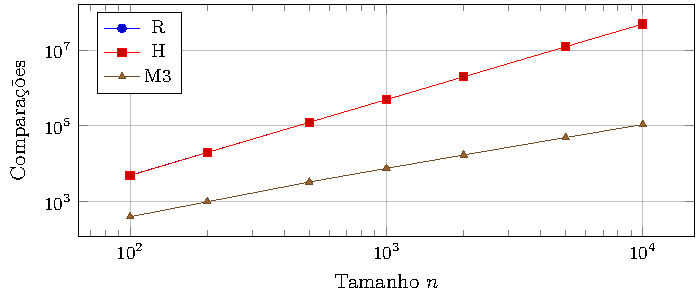
\includegraphics[width=.83\textwidth]{graficos/pior_comparacoes.pdf}
\caption{Comparações médias por tamanho — pior caso explícito}
\label{graf:pior:comparacoes}
\par\smallskip\footnotesize Fonte: arrays\_testados/resultados.csv. Eixos logarítmicos.
\end{grafico}
\begin{table}[htbp]
\centering\small
\caption{Trocas/movimentos médios — pior caso explícito (R, H e M3)}
\label{tab:pior:movimentos}
\begin{tabular}{r r r r}
\hline
$n$ & R & H & M3 \\
\hline
100 & 0 & 0 & 14 \\
200 & 0 & 0 & 30 \\
500 & 0 & 0 & 104 \\
1.000 & 0 & 0 & 208 \\
2.000 & 0 & 0 & 416 \\
5.000 & 0 & 0 & 1.022 \\
10.000 & 0 & 0 & 2.046 \\
\hline
\end{tabular}
\par\smallskip\footnotesize Fonte: arrays\_testados/resultados.csv; contagens médias de operações. H e M3 usam $M=15$.
\end{table}
\begin{grafico}[H]
\centering
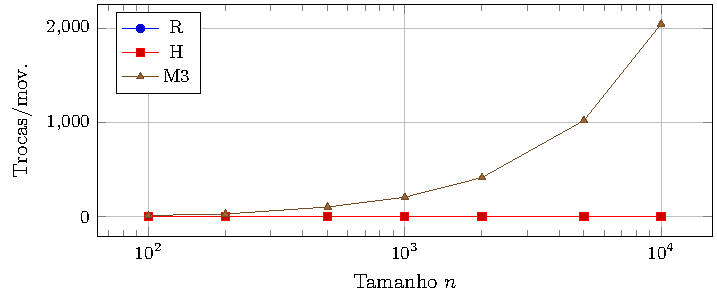
\includegraphics[width=.83\textwidth]{graficos/pior_movimentos.pdf}
\caption{Trocas/movimentos médios por tamanho — pior caso explícito}
\label{graf:pior:movimentos}
\par\smallskip\footnotesize Fonte: arrays\_testados/resultados.csv. Eixo horizontal logarítmico; zero preservado.
\end{grafico}
\subsection*{Interpretação: pior caso explícito com pivô final}
Esta massa é crescente e distinta, como a seção anterior de ordenado, mas foi executada novamente para identificar expressamente o caso adverso de R e H. Em $n=1.000$, R faz 499.500 comparações; em $n=10.000$, 49.995.000: aumentar a entrada dez vezes aumenta as comparações cerca de cem vezes. H faz 49.994.922 comparações em 10.000. M3 faz 108.986 nessa entrada e mantém tempo inferior a 1 ms em todos os tamanhos ensaiados. \emph{Pior caso explícito} designa aqui o pior caso da seleção de pivô final, não um pior caso construído contra M3. As zero trocas de R e H no vetor crescente refletem a convenção de ignorar troca de um índice por ele mesmo; não significam ausência de custo.

